\subsection*{Strømforstærker}
\label{effekt_stroemforstaerker}

\begin{figure}[h]
\centering
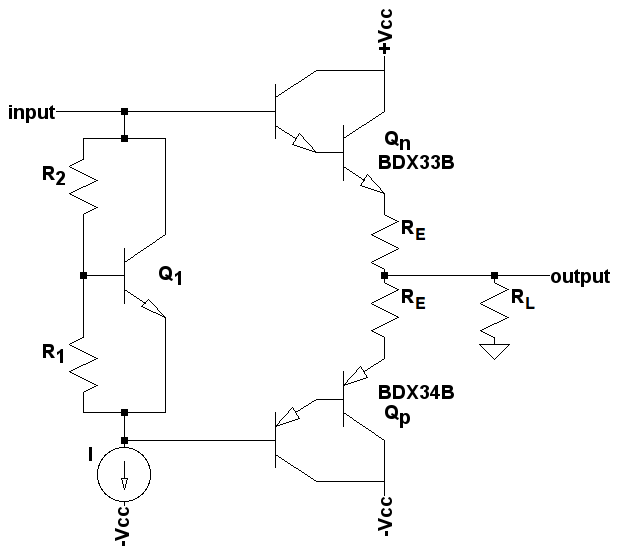
\includegraphics[scale=0.4]{teknisk/effektforstaerker/blokdiagram-stroemforstaerker.png}
\caption{Diagram over strømforstærkeren}
\label{fig:blokdiagram-stroem}
\end{figure}

Strømforstærkeren opbygges som vist på figur \ref{fig:blokdiagram-stroem}. Dog vil konstantstrømsgeneratoren blive bygget i diskret elektronik. Der er valgt at der benyttes en BDX33B og en BDX34B \fixme{kilde: BDX33-34.pdf} som udgangstransistorer. Dette er darlingtontransistorer, som er valgt da de har en $h_{\mathrm{FE}}$ på minimum 750 og kan klare en $I_C$ på op til 10 A. Desuden var de let tilgængelige til projektet.\\
Som vist, i afsnit \ref{valg_kortslutningssikring}, skal der igennem $R_{\mathrm{load}}$ løbe en $I_{\mathrm{peak}}$ på 2,24 A for at opnå en udgangseffekt på 20 W. Dette betyder desuden, som det også er vist i afsnit \ref{valg_kortslutningssikring}, at der skal være en $V_{\mathrm{peak}}$ på 17,9 V over belastningen. %Da de valgte darlingtontransistorer har en $V_{\mathrm{BE}}$ på op til 2,5 V, vælges forsyningsspændingen til $\pm$25 V, hvormed spændingsfaldet over transistorerne ikke umuliggører den tilstrækkelige spænding over belastningen. 
Modstanden $R_E$ bestemmes som det første, udfra termiske hensyn, til 535 m\ohm. Denne udregning kan ses i Appendiks D??. 